\begin{figure}[ht] 
 	\centering 
 	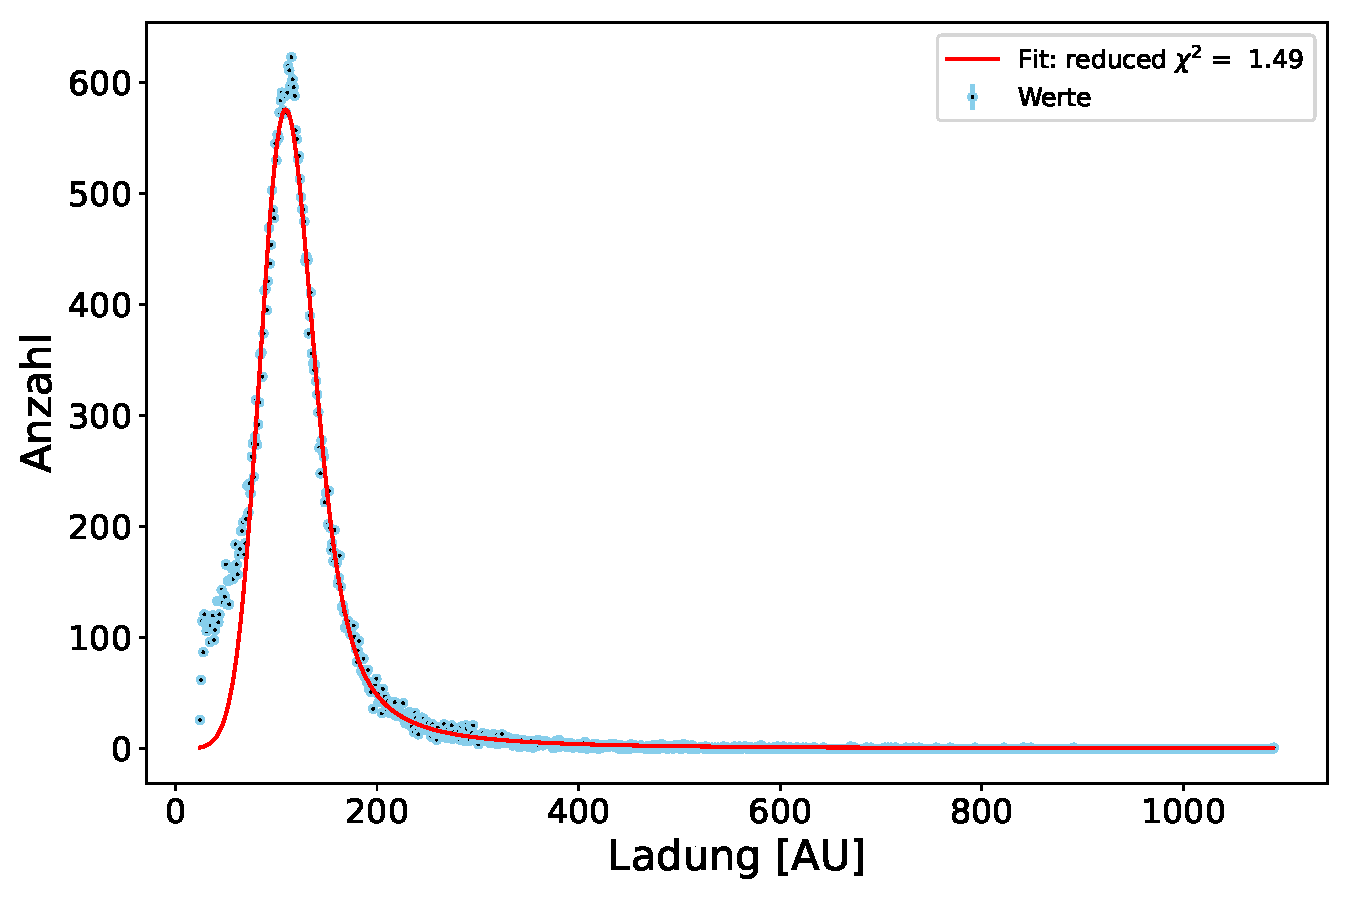
\includegraphics[width= 0.65 \textwidth]{Fits/A4_V40.h5_charge.txt_Fit.pdf} 
	\caption{A4_V40.h5_charge.txt, Fit} 
 	\label{fig:A4_V40.h5_charge.txt, Fit} 
\end{figure}
 \\ 
\begin{table}[ht] 
\centering 
\caption{A4_V40.h5_charge.txt, Fit Parameter Tabelle} 
\label{tab:my-table}
\begin{tabular}{|l|c|}
\hline
Parameter Name	&	Wert \\ \hline
mpv	&	 109.519\\ \hline
eta	&	 7.010\\ \hline
sigma	&	 21.520\\ \hline
A	&	 575.788\\ \hline
\end{tabular} 
\end{table}